\documentclass[11pt,a4paper]{report}

\usepackage[margin=25mm]{geometry}
\usepackage[T1]{fontenc}
\usepackage[utf8]{inputenc}
\usepackage{lmodern}
\usepackage{microtype}
\usepackage{graphicx}
\usepackage{amsmath,amssymb}
\usepackage{booktabs,tabularx,array}
\usepackage{float}
\usepackage{enumitem}
\usepackage{tikz}
\usetikzlibrary{arrows.meta,positioning,shapes.geometric,shapes.multipart,fit,calc}
\usepackage[hidelinks]{hyperref}
\usepackage[section]{placeins}

\setlength{\parindent}{0pt}
\setlength{\parskip}{0.4\baselineskip}
\setcounter{tocdepth}{1}
\setcounter{secnumdepth}{2}
\newcolumntype{Y}{>{\raggedright\arraybackslash}X}
\renewcommand{\arraystretch}{1.15}

\AtBeginDocument{\fontsize{11.25}{13.6}\selectfont}
\tikzset{
  flow/.style={-{Latex[length=2mm]},thick,draw=black},
  component/.style={draw=black,rectangle,rounded corners=2pt,fill=white,
    align=center,font=\small,text width=3.5cm,minimum height=0.95cm},
  usecase/.style={draw=black,ellipse,fill=white,align=center,
    font=\scriptsize,text width=2.55cm,minimum height=0.8cm},
  entity/.style={draw=black,rectangle,fill=white,align=center,
    font=\scriptsize,text width=2.15cm,minimum height=0.65cm},
  decision/.style={draw=black,diamond,aspect=2.1,align=center,
    font=\scriptsize,inner sep=1.2pt,fill=white},
  activity/.style={draw=black,rounded corners=2pt,rectangle,fill=white,
    align=center,font=\scriptsize,text width=3.3cm,minimum height=0.7cm},
  actor/.style={font=\small,align=center}
}

\title{Athena: An AI-Powered Campus Assistant}
\author{Armandeep Singh Taggar -- 1024030219\\
  Sanchit Narula -- 1024031048\\
  Nipun Gupta -- 1024031169\\[0.7em]
  Group 3C73, BE Third Year, Computer Science and Engineering}
\date{November 2026}

\begin{document}
\begin{titlepage}
  \centering
  {\large UCS503P -- Software Engineering Project\par}
  \vspace{1.8cm}
  {\Huge\bfseries Athena\par}
  \vspace{0.45cm}
  {\Large An AI-Powered Campus Assistant\par}
  \vspace{1.5cm}
  {\large Final Project Report\par}
  \vspace{1.1cm}
  {\large Armandeep Singh Taggar -- 1024030219\\[0.2em]
    Sanchit Narula -- 1024031048\\[0.2em]
    Nipun Gupta -- 1024031169\par}
  \vspace{0.5cm}
  {Group 3C73, BE Third Year, Computer Science and Engineering\par}
  \vspace{1cm}
  {Under the guidance of\\[0.2em]
    \large Ms. Jhonsy Bansal\par}
  \vfill
  {\large Computer Science and Engineering Department\\
    Thapar Institute of Engineering and Technology, Patiala\par}
  \vspace{0.45cm}
  {November 2026\par}
\end{titlepage}

\pagenumbering{roman}
\chapter*{Abstract}
Athena is a web-based campus assistant developed to make institutional
information and campus wayfinding easier to access. The final project combines
a React application with a Django REST API, a structured institutional data
model, a question-answering service, and an interactive two-dimensional campus
route finder. The question service matches faculty and course information,
retrieves relevant text from a SQLite FTS5 index, and uses the Google Gemini
API to form a response. The route finder overlays route geometry on a campus
map and provides walking or vehicle directions. The application also contains
pages for account access, academics, societies and events, and student
reminders.

This report describes the implementation found in the submitted project
archive, rather than repeating the earlier proposed architecture. In
particular, the completed code uses FTS5 keyword retrieval rather than
pgvector-based semantic search, and the language-model integration uses Gemini
rather than GPT-4o-mini. A number of interfaces remain demonstrative or use
local mock data. The archive does not contain an automated evaluation dataset,
measured performance results, or a configured production deployment;
accordingly, no numerical accuracy or reliability claims are made. The report
documents these boundaries and identifies practical next steps for testing and
release.

\textbf{Keywords:} campus assistant, retrieval-augmented generation, Django REST,
SQLite FTS5, Gemini API, campus navigation

\tableofcontents
\clearpage
\pagenumbering{arabic}

\chapter{Introduction}

\section{Background}
Students often need to consult several sources to find course information,
faculty contacts, academic rules, events, and campus locations. These sources
may be presented in separate websites, documents, or data tables. A single
interface that supports both questions and navigation can make common campus
tasks easier to start and complete.

Athena addresses this need through a campus-focused web application. It
provides a conversational assistant for institutional questions, pages for
academic and student-life information, and a two-dimensional campus map with
route calculation. Its current data and query logic are centered on Thapar
Institute of Engineering and Technology (TIET); institution records in the
model should not be interpreted as a verified, production-ready
multi-institution service.

\section{Problem Statement}
Campus information is distributed across different sources and may be
difficult to search with a conversational query. Separately, a location name
does not by itself provide a practical route across campus. Athena brings
these tasks together by providing structured information pages, a
 retrieval-backed question service, and an interactive map-based route finder.

\section{Objectives}
The project objectives are to:
\begin{enumerate}[leftmargin=*]
  \item provide a web interface for campus questions and commonly used student
    information;
  \item implement a backend API and persistent domain model for institutions,
    students, academic records, buildings, events, societies, and reminders;
  \item retrieve relevant institutional text and generate a conversational
    answer, including source references when requested;
  \item support campus route planning with a map overlay and walking or vehicle
    modes; and
  \item assess the implemented scope honestly and identify remaining testing,
    security, and deployment work.
\end{enumerate}

\section{Scope of the Final Implementation}
The repository contains a React/Vite frontend, a Django and Django REST
Framework backend, ORM models and migrations, frontend fallback data, and a
standalone campus navigation page embedded in the application. The assistant
uses an SQLite FTS5 index and a Gemini API integration. PostgreSQL is supported
as a configured database option for the Django application, with local SQLite
as a fallback.

The submitted code does not implement the prototype report's proposed
Sentence-Transformers embeddings, pgvector retrieval, PyMuPDF ingestion, or
GPT-4o-mini integration. It also does not establish that every student-life
interface is backed by live data, that email ownership is verified, or that a
production deployment has been completed. Chapter~\ref{chap:status}
separates working code paths from mock or incomplete parts.

\chapter{Requirements and System Design}

\section{Functional Requirements}
The implemented application provides the following user-facing functions:
\begin{itemize}[leftmargin=*]
  \item select an institution, create a student account, and sign in;
  \item ask a natural-language question and display an answer with optional
    source chips or a location action;
  \item browse course and faculty information and use the CGPA calculator;
  \item browse society and event listings;
  \item open a campus map and request a route between listed places; and
  \item view a dashboard with reminder controls and an institutional document
    registry screen.
\end{itemize}

The last item needs qualification: reminders use a frontend mock module in the
submitted code, and the document registry's upload and removal controls are
not connected to a document-ingestion API. They are included in the interface,
but should not be reported as completed persistent services.

\section{Non-Functional Requirements}
The design is modular, with a browser client, REST API, database-backed domain
models, local full-text search, and an external language-model service.
Configuration is environment-driven for database URLs, API credentials,
allowed hosts, and cross-origin settings. Security, answer quality,
availability, and response time still require systematic validation. The
report makes no claim that these properties have been measured or achieved in
production.

\clearpage
\section{Architecture}
Figure~\ref{fig:architecture} summarizes the architecture visible in the
submitted source. Structured records are served through Django REST endpoints.
The query endpoint calls a Python service that combines structured faculty and
course matching, document retrieval from SQLite FTS5, and Gemini response
generation. The standalone route finder runs in the browser and is embedded
within the React application. The Django configuration can use PostgreSQL or
SQLite; the FTS5 document index is a separate SQLite store.

\begin{figure}[htbp]
\centering
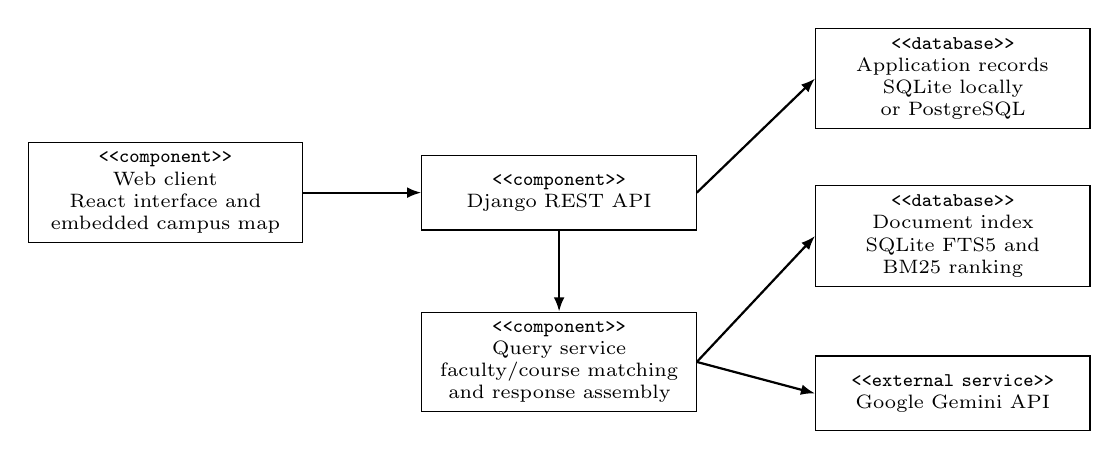
\begin{tikzpicture}[
  component/.style={draw=black,rectangle,fill=white,align=center,
    font=\scriptsize,text width=3.25cm,minimum height=0.95cm},
  dependency/.style={-{Latex[length=1.8mm]},thick,draw=black}
]
  \node[component] (client) at (-5,0)
    {\texttt{<<component>>}\\Web client\\React interface and embedded campus map};
  \node[component] (api) at (0,0)
    {\texttt{<<component>>}\\Django REST API};
  \node[component] (query) at (0,-2.15)
    {\texttt{<<component>>}\\Query service\\faculty/course matching and response assembly};
  \node[component] (database) at (5,1.45)
    {\texttt{<<database>>}\\Application records\\SQLite locally or PostgreSQL};
  \node[component] (fts) at (5,-0.55)
    {\texttt{<<database>>}\\Document index\\SQLite FTS5 and BM25 ranking};
  \node[component] (gemini) at (5,-2.55)
    {\texttt{<<external service>>}\\Google Gemini API};

  \draw[dependency] (client.east) -- (api.west);
  \draw[dependency] (api.east) -- (database.west);
  \draw[dependency] (api.south) -- (query.north);
  \draw[dependency] (query.east) -- (fts.west);
  \draw[dependency] (query.east) -- (gemini.west);
\end{tikzpicture}
\caption{UML component view of the browser client, API, query service, data stores, and external model. Solid arrows show dependency direction.}
\label{fig:architecture}
\end{figure}

\section{Technology Stack}
\begin{table}[htbp]
\centering
\small
\begin{tabularx}{\linewidth}{@{}p{2.7cm}p{4cm}Y@{}}
\toprule
\textbf{Area} & \textbf{Implementation in repository} & \textbf{Role} \\
\midrule
Frontend & React, Vite, Tailwind CSS & Pages, assistant interface, data views, and route-map embedding. \\
Backend & Python, Django, Django REST Framework & Authentication, API endpoints, serializers, and application logic. \\
Domain data & Django ORM; SQLite default with PostgreSQL configuration & Institution, student, department, course, faculty, building, room, event, society, document, and reminder records. \\
Document retrieval & SQLite FTS5 & Full-text indexing and BM25-ranked retrieval of prepared text chunks. \\
Answer generation & Google Gemini API & Produces a response from the question and retrieved/structured context; a direct fallback is provided for API failure. \\
Campus routing & JavaScript, SVG, campus-map image & Draws route overlays and presents walking or vehicle directions. \\
\bottomrule
\end{tabularx}
\caption{Implemented technology choices; this table does not imply production validation.}
\label{tab:stack}
\end{table}

\clearpage
\section{Use Case Diagram}
Figure~\ref{fig:usecase} reflects the visible student and administrator
interactions. The document-registry use case represents a static screen; its
upload and removal controls are not connected to an ingestion service. Email
checking compares a domain string and does not confirm mailbox ownership.

\begin{figure}[H]
\centering
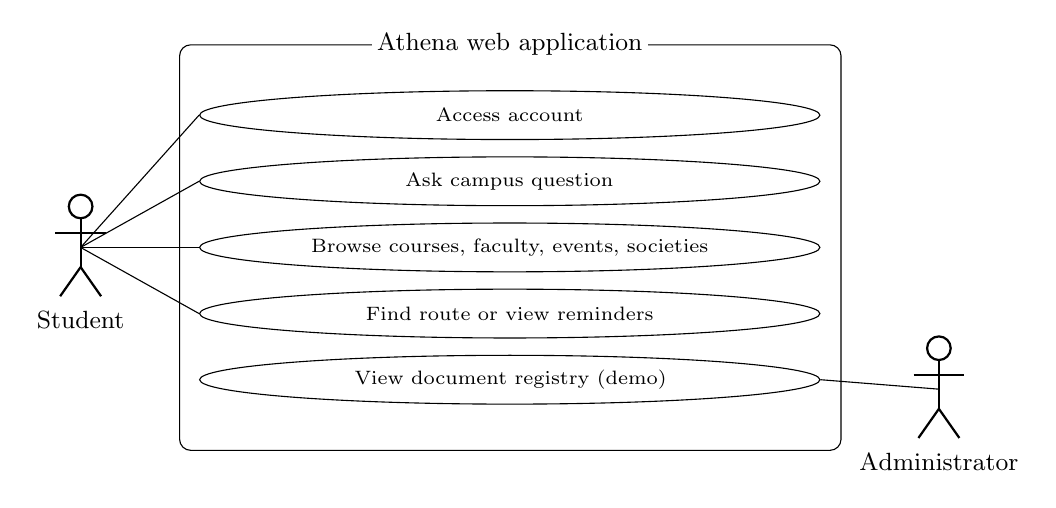
\begin{tikzpicture}[
  association/.style={draw=black,thin},
  case/.style={draw=black,ellipse,fill=white,align=center,
    font=\scriptsize,text width=5.5cm,minimum height=0.62cm,inner sep=1pt},
  actorline/.style={draw=black,thick},
  actorlabel/.style={font=\small,align=center}
]
  \node[draw=black,rounded corners,minimum width=8.4cm,minimum height=5.15cm,
    anchor=north west] (system) at (-4.2,2.58) {};
  \node[font=\small,fill=white,inner sep=2pt] at (0,2.58)
    {Athena web application};

  \coordinate (student) at (-5.45,0);
  \draw[actorline] ($(student)+(0,0.52)$) circle (0.15);
  \draw[actorline] ($(student)+(0,0.37)$) -- ($(student)+(0,-0.25)$);
  \draw[actorline] ($(student)+(-0.32,0.18)$) -- ($(student)+(0.32,0.18)$);
  \draw[actorline] ($(student)+(0,-0.25)$) -- ($(student)+(-0.26,-0.62)$);
  \draw[actorline] ($(student)+(0,-0.25)$) -- ($(student)+(0.26,-0.62)$);
  \node[actorlabel] at (-5.45,-0.92) {Student};

  \coordinate (administrator) at (5.45,-1.8);
  \draw[actorline] ($(administrator)+(0,0.52)$) circle (0.15);
  \draw[actorline] ($(administrator)+(0,0.37)$) -- ($(administrator)+(0,-0.25)$);
  \draw[actorline] ($(administrator)+(-0.32,0.18)$) -- ($(administrator)+(0.32,0.18)$);
  \draw[actorline] ($(administrator)+(0,-0.25)$) -- ($(administrator)+(-0.26,-0.62)$);
  \draw[actorline] ($(administrator)+(0,-0.25)$) -- ($(administrator)+(0.26,-0.62)$);
  \node[actorlabel] at (5.45,-2.72) {Administrator};

  \node[case] (account) at (0,1.68) {Access account};
  \node[case] (assistant) at (0,0.84) {Ask campus question};
  \node[case] (information) at (0,0) {Browse courses, faculty, events, societies};
  \node[case] (campus) at (0,-0.84) {Find route or view reminders};
  \node[case] (documents) at (0,-1.68) {View document registry (demo)};

  \draw[association] (student) -- (account.west);
  \draw[association] (student) -- (assistant.west);
  \draw[association] (student) -- (information.west);
  \draw[association] (student) -- (campus.west);
  \draw[association] (administrator) -- (documents.east);
\end{tikzpicture}
\caption{UML use-case diagram. Actor associations are unarrowed; the email check uses domain matching, while reminders and document administration remain incomplete or mock-backed.}
\label{fig:usecase}
\end{figure}

\section{Domain Class Diagram}
Figure~\ref{fig:class} uses UML class compartments and unarrowed associations
with multiplicities to show the principal Django model relationships. The
selected classes include representative attributes; \texttt{Admin},
\texttt{Event}, \texttt{Society}, \texttt{SocietyMember}, and
\texttt{KnowledgeDocument} are omitted to keep the model readable. The FTS5
index is populated from JSONL data rather than managed through the document
model.

\begin{figure}[H]
\centering
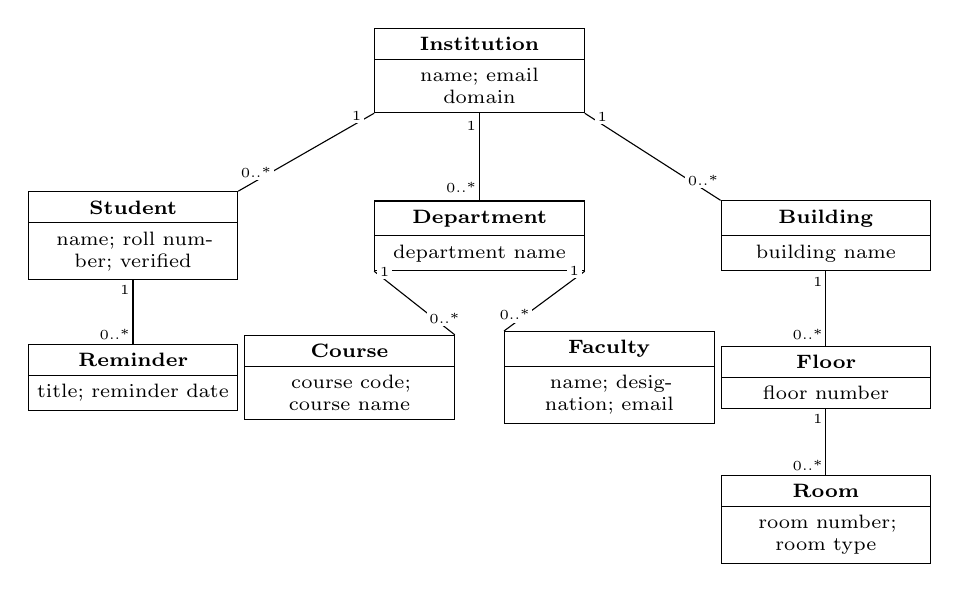
\begin{tikzpicture}[
  classbox/.style={rectangle split,rectangle split parts=2,draw=black,
    fill=white,align=center,font=\scriptsize,text width=2.45cm,
    minimum height=1.05cm,inner sep=3pt},
  association/.style={draw=black,thin},
  multiplicity/.style={font=\tiny,fill=white,inner sep=1pt}
]
  \node[classbox] (institution) at (0,2.6)
    {\textbf{Institution}\nodepart{second}name; email domain};
  \node[classbox] (student) at (-4.4,0.5)
    {\textbf{Student}\nodepart{second}name; roll number; verified};
  \node[classbox] (department) at (0,0.5)
    {\textbf{Department}\nodepart{second}department name};
  \node[classbox] (building) at (4.4,0.5)
    {\textbf{Building}\nodepart{second}building name};
  \node[classbox] (reminder) at (-4.4,-1.3)
    {\textbf{Reminder}\nodepart{second}title; reminder date};
  \node[classbox] (course) at (-1.65,-1.3)
    {\textbf{Course}\nodepart{second}course code; course name};
  \node[classbox] (faculty) at (1.65,-1.3)
    {\textbf{Faculty}\nodepart{second}name; designation; email};
  \node[classbox] (floor) at (4.4,-1.3)
    {\textbf{Floor}\nodepart{second}floor number};
  \node[classbox] (room) at (4.4,-3.1)
    {\textbf{Room}\nodepart{second}room number; room type};

  \draw[association] (institution.south west) -- (student.north east)
    node[multiplicity,pos=0.13,above] {1}
    node[multiplicity,pos=0.87,above] {0..*};
  \draw[association] (institution.south) -- (department.north)
    node[multiplicity,pos=0.15,left] {1}
    node[multiplicity,pos=0.85,left] {0..*};
  \draw[association] (institution.south east) -- (building.north west)
    node[multiplicity,pos=0.13,above] {1}
    node[multiplicity,pos=0.87,above] {0..*};
  \draw[association] (student.south) -- (reminder.north)
    node[multiplicity,pos=0.15,left] {1}
    node[multiplicity,pos=0.85,left] {0..*};
  \draw[association] (department.south west) -- (course.north east)
    node[multiplicity,pos=0.13,above] {1}
    node[multiplicity,pos=0.87,above] {0..*};
  \draw[association] (department.south east) -- (faculty.north west)
    node[multiplicity,pos=0.13,above] {1}
    node[multiplicity,pos=0.87,above] {0..*};
  \draw[association] (building.south) -- (floor.north)
    node[multiplicity,pos=0.15,left] {1}
    node[multiplicity,pos=0.85,left] {0..*};
  \draw[association] (floor.south) -- (room.north)
    node[multiplicity,pos=0.15,left] {1}
    node[multiplicity,pos=0.85,left] {0..*};
\end{tikzpicture}
\caption{UML class diagram showing selected model attributes and one-to-many associations.}
\label{fig:class}
\end{figure}

\section{Assistant Activity Diagram}
Figure~\ref{fig:activity} presents the implemented query path at a useful
level of detail. The service performs specialized faculty/course matching and
document retrieval, detects supported location keywords, and calls Gemini.
When the external call is unavailable, the service attempts a direct fallback
using the matched information or a retrieved passage.

\begin{figure}[H]
\centering
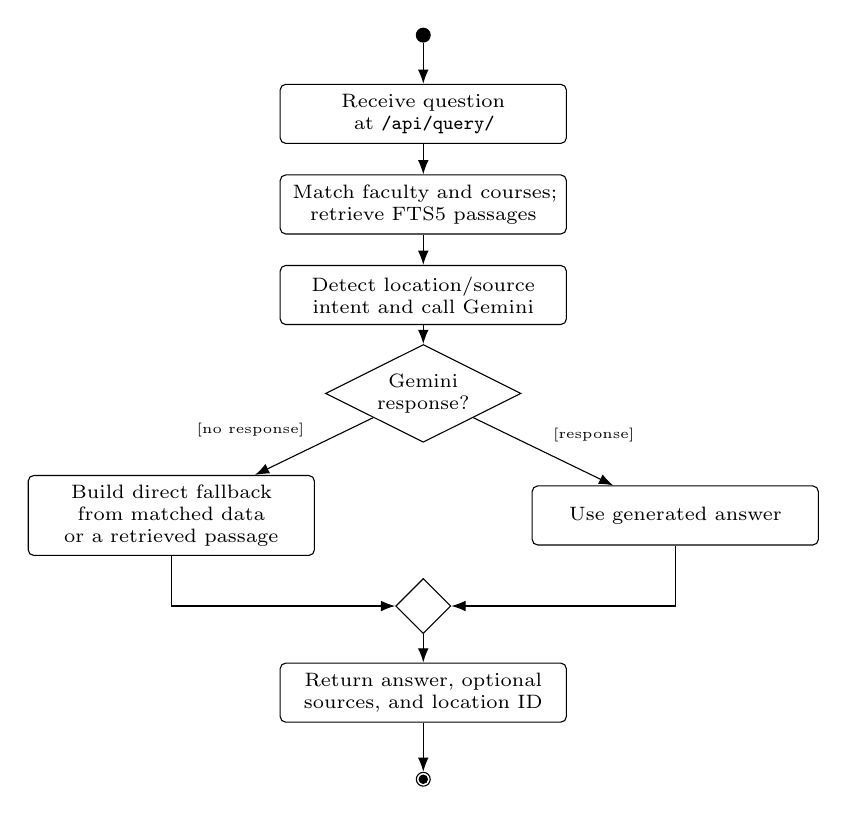
\begin{tikzpicture}[
  action/.style={draw=black,rounded corners=2pt,rectangle,fill=white,
    align=center,font=\scriptsize,text width=3.4cm,minimum height=0.75cm},
  decision/.style={draw=black,diamond,aspect=2.0,align=center,
    font=\scriptsize,minimum size=9pt,inner sep=1.5pt,fill=white},
  control/.style={-{Latex[length=1.8mm]},thin,draw=black},
  mergepoint/.style={draw=black,diamond,minimum size=7mm,inner sep=0pt,fill=white}
]
  \node[draw=black,circle,fill=black,minimum size=5pt,inner sep=0pt] (start) at (0,0) {};
  \node[action] (receive) at (0,-1.0) {Receive question at \texttt{/api/query/}};
  \node[action] (retrieve) at (0,-2.15) {Match faculty and courses; retrieve FTS5 passages};
  \node[action] (generate) at (0,-3.3) {Detect location/source intent and call Gemini};
  \node[decision] (available) at (0,-4.55) {Gemini\\response?};
  \node[action] (fallback) at (-3.2,-6.1) {Build direct fallback from matched data or a retrieved passage};
  \node[action] (answer) at (3.2,-6.1) {Use generated answer};
  \node[mergepoint] (merge) at (0,-7.25) {};
  \node[action] (format) at (0,-8.35) {Return answer, optional sources, and location ID};
  \node[draw=black,circle,minimum size=5pt,inner sep=0pt] (final) at (0,-9.45) {};
  \node[draw=black,circle,fill=black,minimum size=3pt,inner sep=0pt] at (0,-9.45) {};

  \draw[control] (start) -- (receive);
  \draw[control] (receive) -- (retrieve);
  \draw[control] (retrieve) -- (generate);
  \draw[control] (generate) -- (available);
  \draw[control] (available) -- node[above left,font=\tiny,fill=white] {[no response]} (fallback);
  \draw[control] (available) -- node[above right,font=\tiny,fill=white] {[response]} (answer);
  \draw[control] (fallback.south) |- (merge.west);
  \draw[control] (answer.south) |- (merge.east);
  \draw[control] (merge) -- (format);
  \draw[control] (format) -- (final);
\end{tikzpicture}
\caption{UML activity diagram. Guard conditions label the decision branches; the diamond below merges the two answer paths.}
\label{fig:activity}
\end{figure}

The diagram starts when the API receives a question, then shows the service
checking structured faculty/course cases, retrieving FTS5 passages, and
checking location or source intent before generation. The decision guard
separates a generated answer from the direct fallback; both paths rejoin before
the response is formatted. Source references and a location identifier are
optional response details, not proof of retrieval or answer accuracy.

\clearpage
\section{Query Sequence Diagram}
Figure~\ref{fig:sequence} shows the principal interactions for an assistant
query. Source metadata is included in the response only when the query is
recognized as explicitly requesting references. Location detection returns an
identifier; map display is a separate frontend action.

\begin{figure}[H]
\centering
\resizebox{\linewidth}{!}{%
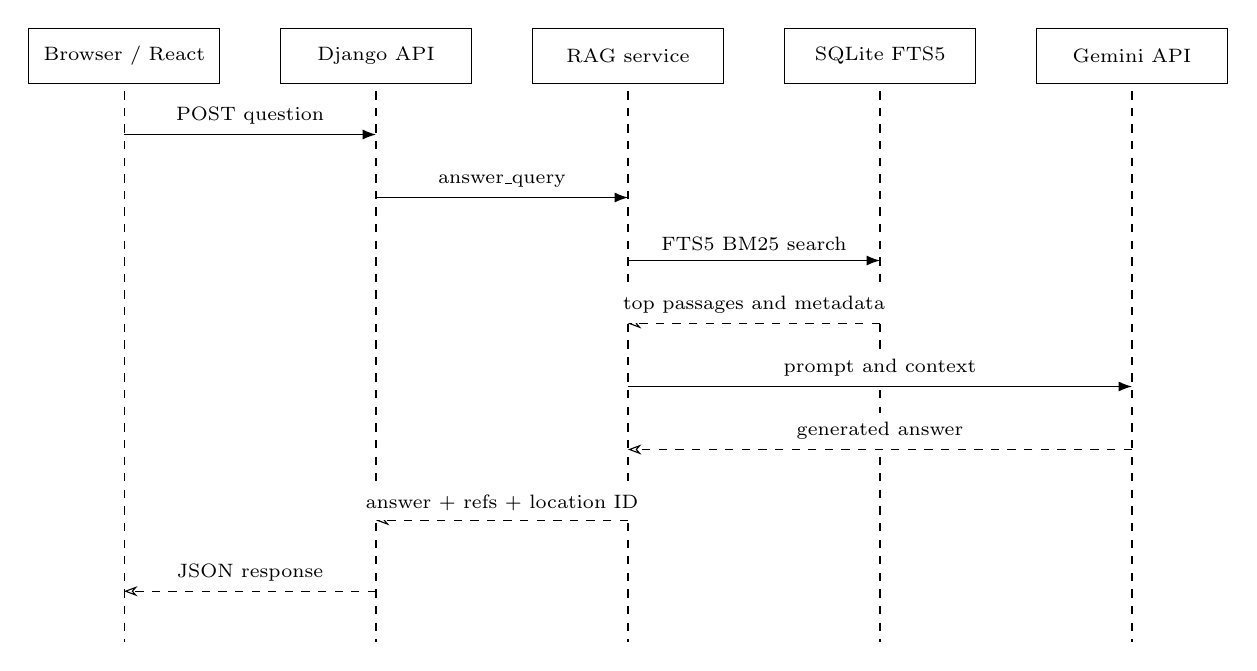
\begin{tikzpicture}[
  participant/.style={draw=black,rectangle,fill=white,align=center,
    font=\scriptsize,text width=2.2cm,minimum height=0.7cm},
  message/.style={-{Latex[length=1.7mm]},thin,draw=black},
  reply/.style={-{Stealth[open,length=1.7mm]},thin,dashed,draw=black}
]
  \node[participant] (browser) at (0,0) {Browser / React};
  \node[participant] (api) at (3.2,0) {Django API};
  \node[participant] (service) at (6.4,0) {RAG service};
  \node[participant] (fts) at (9.6,0) {SQLite FTS5};
  \node[participant] (gemini) at (12.8,0) {Gemini API};
  \foreach \x in {0,3.2,6.4,9.6,12.8} {
    \draw[dashed,thin] (\x,-0.45) -- (\x,-7.45);
  }

  \draw[message] (0,-1.0) -- node[above,font=\scriptsize,fill=white] {POST question} (3.2,-1.0);
  \draw[message] (3.2,-1.8) -- node[above,font=\scriptsize,fill=white] {answer\_query} (6.4,-1.8);
  \draw[message] (6.4,-2.6) -- node[above,font=\scriptsize,fill=white] {FTS5 BM25 search} (9.6,-2.6);
  \draw[reply] (9.6,-3.4) -- node[above,font=\scriptsize,fill=white] {top passages and metadata} (6.4,-3.4);
  \draw[message] (6.4,-4.2) -- node[above,font=\scriptsize,fill=white] {prompt and context} (12.8,-4.2);
  \draw[reply] (12.8,-5.0) -- node[above,font=\scriptsize,fill=white] {generated answer} (6.4,-5.0);
  \draw[reply] (6.4,-5.9) -- node[above,font=\scriptsize,fill=white] {answer + refs + location ID} (3.2,-5.9);
  \draw[reply] (3.2,-6.8) -- node[above,font=\scriptsize,fill=white] {JSON response} (0,-6.8);
\end{tikzpicture}%
}
\caption{UML sequence diagram. Solid arrows are calls; dashed arrows are returned results.}
\label{fig:sequence}
\end{figure}

Read the sequence from top to bottom: the browser posts the question, Django
invokes the RAG service, and that service retrieves passages before sending the
question and context to Gemini. The returned answer travels back through the
service and API to the browser. This is the normal generation path; the
activity diagram shows the fallback when Gemini does not return a response.
Source references appear only for recognized requests, and a detected location
ID can trigger a separate map action in the frontend.

\chapter{Implementation}

\section{Frontend}
The frontend is a React application built with Vite and styled using Tailwind
CSS. React Router separates the landing page, institution selection, login and
registration, dashboard, academics, society/events, navigation, and document
registry pages. An authentication context stores the returned token and user
information in browser local storage; a route wrapper redirects unauthenticated
users away from selected pages.

The dashboard exposes navigation tiles, a floating assistant, and reminders.
The academics page displays courses and faculty and includes timetable,
date-sheet, and CGPA-related components. The society and events page loads
listings through API helper modules with local mock fallbacks. Reminder data is
currently held by the frontend mock module rather than persisted via the
backend reminder endpoint.

\section{Backend and Data Model}
The backend uses Django and Django REST Framework~\cite{drfdocs}. Its API includes registration
and login, institution/course/faculty/event/society/map-location listing,
student reminders, and the assistant query endpoint. Token authentication is
configured for authenticated requests. The Django models define institutions,
student and administrator profiles, departments, courses, faculty, buildings,
floors, rooms, events, knowledge-document metadata, societies, memberships,
and reminders.

The backend settings support a database URL or discrete database connection
variables, and fall back to a local SQLite database when these are not
provided. The ORM schema and the assistant's document index are distinct:
the latter is an SQLite FTS5 database built from prepared JSON Lines chunks.

\section{Question Answering}
The endpoint \texttt{POST /api/query/} calls \texttt{TIETRAGService}, which
checks faculty and course/CGPA queries, retrieves passages from SQLite FTS5
using BM25~\cite{sqlitefts5}, and detects campus-location keywords. It sends the
question and available structured or retrieved context to Gemini~\cite{geminiapi};
if generation fails, it falls back to matched records or the first passage.
Responses contain an answer, optional source list, and optional location ID.
This is keyword-based retrieval, not semantic vector search~\cite{lewis2020rag}.
The service expects JSONL data in the backend's \texttt{ThaparInfo} directory,
which is absent from the archive; a working instance also requires a Gemini key
and seeded structured records.

\section{Campus Navigation}
The React navigation page embeds a standalone HTML/JavaScript route finder. It
uses campus place and road-graph data, overlays SVG routes on a map image, and
supports endpoint selection, walking or vehicle modes, zoom, pan, and directions.
The journals record fixes to connectivity, road snapping, and map alignment, but
do not provide systematic route tests.

\section{Deployment View}
The source configures separate browser and Django applications, database
options, and a backend Gemini credential. No release workflow or verified
production instance is included; Figure~\ref{fig:runtime} shows runtime nodes,
not deployed hosting.

\begin{figure}[htbp]
\centering
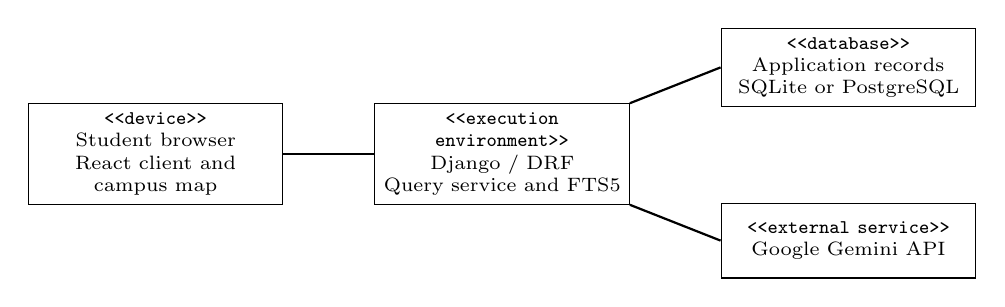
\begin{tikzpicture}[
  nodebox/.style={draw=black,rectangle,fill=white,align=center,
    font=\scriptsize,text width=3.0cm,minimum height=0.95cm},
  comm/.style={draw=black,thick}
]
  \node[nodebox] (browser) at (-4.4,0)
    {\texttt{<<device>>}\\Student browser\\React client and campus map};
  \node[nodebox] (server) at (0,0)
    {\texttt{<<execution environment>>}\\Django / DRF\\Query service and FTS5};
  \node[nodebox] (database) at (4.4,1.1)
    {\texttt{<<database>>}\\Application records\\SQLite or PostgreSQL};
  \node[nodebox] (gemini) at (4.4,-1.1)
    {\texttt{<<external service>>}\\Google Gemini API};

  \draw[comm] (browser.east) -- (server.west);
  \draw[comm] (server.north east) -- (database.west);
  \draw[comm] (server.south east) -- (gemini.west);
\end{tikzpicture}
\caption{UML deployment view of runtime nodes and communication paths; no hosting provider is asserted.}
\label{fig:runtime}
\end{figure}

\section{Software Development Life Cycle}
The prototype report presents an iterative lifecycle~\cite{prototype-report}.
This adaptation reflects the archive's manual implementation and review; it
does not assert configured CI/CD, staging, or production release.

\begin{figure}[H]
\centering
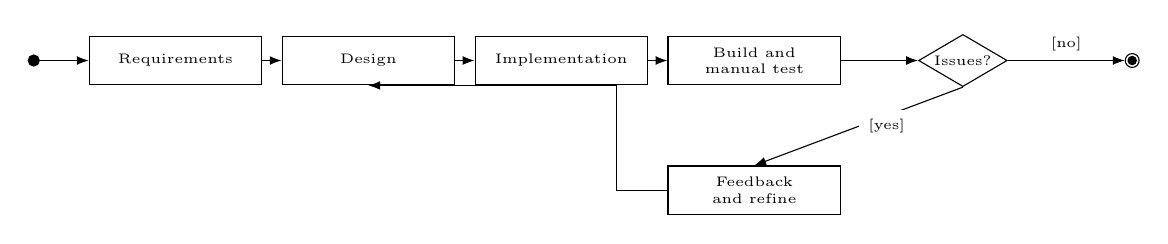
\begin{tikzpicture}[
  phase/.style={draw=black,rectangle,fill=white,align=center,
    font=\tiny,text width=2.05cm,minimum height=0.62cm,inner sep=2pt},
  gate/.style={draw=black,diamond,aspect=1.7,align=center,
    font=\tiny,inner sep=1pt},
  control/.style={-{Latex[length=1.5mm]},thin,draw=black}
]
  \node[draw=black,circle,fill=black,minimum size=4pt,inner sep=0pt] (start) at (-7.15,0) {};
  \node[phase] (requirements) at (-5.35,0) {Requirements};
  \node[phase] (design) at (-2.9,0) {Design};
  \node[phase] (implementation) at (-0.45,0) {Implementation};
  \node[phase] (testing) at (2.0,0) {Build and manual test};
  \node[gate] (review) at (4.65,0) {Issues?};
  \node[phase] (refine) at (2.0,-1.65) {Feedback and refine};
  \node[draw=black,circle,minimum size=5pt,inner sep=0pt] (finish) at (6.8,0) {};
  \node[draw=black,circle,fill=black,minimum size=3pt,inner sep=0pt] at (6.8,0) {};

  \draw[control] (start) -- (requirements);
  \draw[control] (requirements) -- (design);
  \draw[control] (design) -- (implementation);
  \draw[control] (implementation) -- (testing);
  \draw[control] (testing) -- (review);
  \draw[control] (review.east) -- node[above,font=\tiny,fill=white] {[no]} (finish);
  \draw[control] (review.south) -- node[right,font=\tiny,fill=white] {[yes]} (refine.north);
  \draw[control] (refine.west) -- ++(-0.65,0) |- (design.south);
\end{tikzpicture}
\caption{Monochrome UML activity view adapted from the prototype lifecycle. The feedback loop represents iterative refinement, not an automated release pipeline.}
\label{fig:sdlc}
\end{figure}

\chapter{Results and Evaluation}
\label{chap:status}

\section{Implementation Status}
The table summarizes evidence in the submitted source archive~\cite{athena-source},
distinguishing code paths from end-to-end verification.

\begin{table}[htbp]
\centering
\small
\begin{tabularx}{\linewidth}{@{}p{3.3cm}p{2.4cm}Y@{}}
\toprule
\textbf{Feature} & \textbf{Status} & \textbf{Evidence and qualification} \\
\midrule
React web application & Implemented & Routes and components exist for the landing, account, dashboard, academic, student-life, and navigation screens. \\
Django REST API & Implemented & Auth and read endpoints plus a query endpoint are present. Database setup and seeded data are required for useful live results. \\
Question answering & Implemented, data-dependent & FTS5 retrieval and Gemini generation are coded; the expected knowledge-base data directory and API credential are not included in the archive. \\
Campus route finder & Implemented & Standalone JavaScript/HTML page calculates routes and renders them over a map. Route correctness is not covered by an automated test suite. \\
Email affiliation & Partial & The frontend checks the email's domain string; the backend restricts registration to \texttt{@thapar.edu}. No mailbox ownership confirmation is implemented. \\
Academic, event, society listings & Partial & API endpoints and frontend helpers exist; fallback JSON data is used when requests fail, so a screen can appear populated without live backend data. \\
Reminders & Partial & A Django model and endpoint exist, but the frontend reminder helper uses in-memory mock data. \\
Automated evaluation/deployment & Partial evidence & Manual functional and integration checks were performed during development; automated test files remain placeholders, and no release workflow or production deployment is documented in the archive. \\
\bottomrule
\end{tabularx}
\caption{Code-level implementation status based on the submitted project archive.}
\label{tab:status}
\end{table}

\section{Manual Checks}
Manual functional and integration checks were carried out while the frontend,
backend, assistant, and campus map were developed. The team journals record
route review and iterative fixes; the checks below summarize the documented
scope without implying a formal user study or measured performance test.

\begin{table}[htbp]
\centering
\small
\begin{tabularx}{\linewidth}{@{}p{3.0cm}p{5.0cm}Y@{}}
\toprule
\textbf{Area} & \textbf{Manual check} & \textbf{Observed result} \\
\midrule
Frontend/backend integration & Reviewed application behavior as the React interface, Django API, assistant, and campus map were connected. & Integration was reviewed during development; detailed inputs and case-by-case pass/fail records are not preserved. \\
Campus route connectivity & Reviewed route-graph connectivity and route behavior on the campus map. & Connectivity issues were identified during development and addressed iteratively; no route-success percentage was measured. \\
Road snapping & Checked how route points snapped to the mapped road network. & Snapping issues were recorded and fixed iteratively; a complete repeatable test log is not available. \\
Map alignment & Reviewed alignment of route overlays with the campus map. & Alignment issues were addressed during development; no systematic calibration measurements are documented. \\
\bottomrule
\end{tabularx}
\caption{Summary of manual checks documented during development.}
\label{tab:manual-checks}
\end{table}

\section{CodeCheck Results}
The supplied Django test-run output reports 11 tests, all passing in 0.157
seconds. Table~\ref{tab:codecheck} lists the cases and outcomes. These results
cover the named registration, serializer, and API endpoint checks; they do not
measure route correctness, answer quality, frontend behavior, or system
performance.

\begin{table}[htbp]
\centering
\scriptsize
\begin{tabularx}{\linewidth}{@{}p{3.3cm}Yp{1.3cm}@{}}
\toprule
\textbf{Test ID} & \textbf{Code check} & \textbf{Result} \\
\midrule
TC\_AUTH\_01 & Valid \texttt{@thapar.edu} registration succeeds. & PASS \\
TC\_AUTH\_02 & Registration with a non-Thapar email (for example, \texttt{@gmail.com}) is rejected with a validation error. & PASS \\
TC\_AUTH\_03 & Duplicate email registration is rejected. & PASS \\
TC\_SERIALIZER\_01 & Institution serializer provides the \texttt{domain} alias for \texttt{email\_domain}. & PASS \\
TC\_SERIALIZER\_02 & Event serializer provides title, date, and venue aliases. & PASS \\
TC\_SERIALIZER\_03 & Society serializer provides the \texttt{name} alias for \texttt{society\_name}. & PASS \\
TC\_SERIALIZER\_04 & Faculty serializer correctly maps \texttt{departmentCode}. & PASS \\
TC\_API\_01 & \texttt{GET /api/institutions/} returns HTTP 200. & PASS \\
TC\_API\_02 & \texttt{GET /api/faculty/} returns HTTP 200. & PASS \\
TC\_API\_03 & \texttt{GET /api/societies/} returns HTTP 200. & PASS \\
TC\_API\_04 & \texttt{GET /api/events/} returns HTTP 200. & PASS \\
\bottomrule
\end{tabularx}
\caption{Automated Django code-check results from the supplied test output (11 of 11 passed).}
\label{tab:codecheck}
\end{table}

The reported test run provides automated evidence for these backend checks.
It is not a substitute for controlled performance runs, a structured student
study, route tests, or evaluation against a labelled question-answer corpus.

\section{Limitations and Risks}
\begin{enumerate}[leftmargin=*]
  \item \textbf{Institution coverage:} registration and knowledge matching
    contain TIET-specific assumptions. Institution records alone do not provide
    tested cross-institution data isolation or onboarding.
  \item \textbf{Operational readiness:} credentials, required data files,
    migrations, CORS/host settings, monitoring, and release procedures must be
    configured for a deployment. Production availability has not been
    demonstrated by the archive.
  \item \textbf{Additional threats to validity:} Serverless cold starts can
    dominate latency; increasing a timeout avoids premature cancellation but
    does not improve responsiveness. Map calibration and source geometry affect
    snapping, and a connected graph can still omit a real walkway. RAG coverage,
    chunking, and refresh frequency constrain answers; stale approved documents
    can still produce stale responses. Without a ground-truth corpus and
    repeated performance runs, numerical quality and production-latency claims
    are unsupported. Domain syntax alone does not prove mailbox control.
    Source provenance and expiry, route audits, ownership verification, and
    reproducible evaluation sets mitigate these threats.
\end{enumerate}

\clearpage





\section{Development Process}
The team journals record incremental work on project selection, schema and
backend development, frontend integration, and campus routing.
Figure~\ref{fig:process} shows the resulting iterative process at a high
level; it does not imply a configured CI/CD pipeline.

\begin{figure}[htbp]
\centering
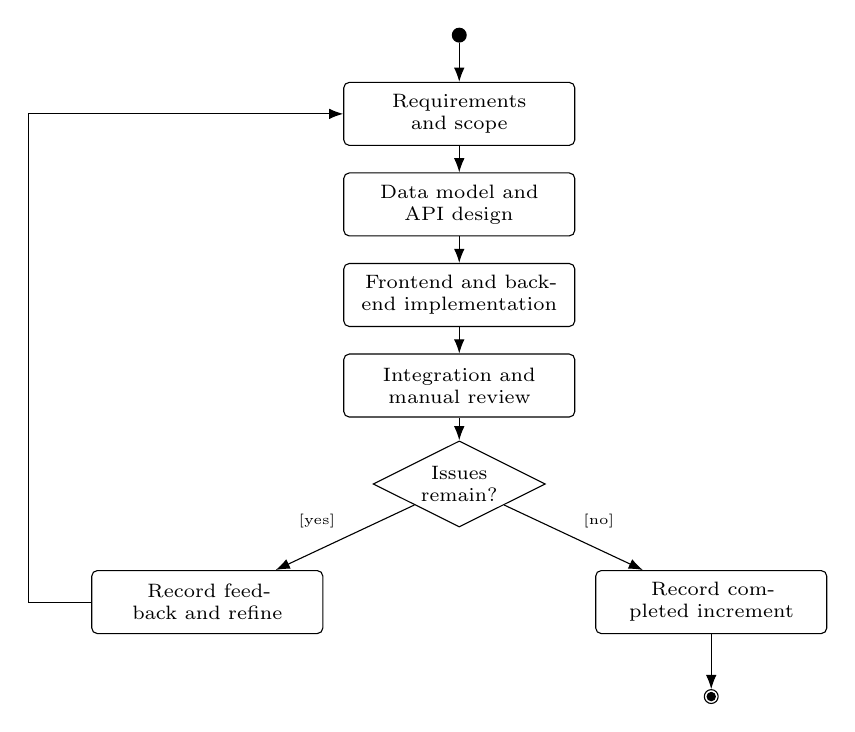
\begin{tikzpicture}[
  action/.style={draw=black,rounded corners=2pt,rectangle,fill=white,
    align=center,font=\scriptsize,text width=2.7cm,minimum height=0.8cm},
  decision/.style={draw=black,diamond,aspect=2.0,align=center,
    font=\scriptsize,minimum size=9pt,inner sep=1.5pt,fill=white},
  control/.style={-{Latex[length=1.8mm]},thin,draw=black},
  mergepoint/.style={draw=black,diamond,minimum size=7mm,inner sep=0pt,fill=white}
]
  \node[draw=black,circle,fill=black,minimum size=5pt,inner sep=0pt] (start) at (0,0) {};
  \node[action] (requirements) at (0,-1.0) {Requirements and scope};
  \node[action] (design) at (0,-2.15) {Data model and API design};
  \node[action] (implementation) at (0,-3.3) {Frontend and backend implementation};
  \node[action] (review) at (0,-4.45) {Integration and manual review};
  \node[decision] (issues) at (0,-5.7) {Issues\\remain?};
  \node[action] (refine) at (-3.2,-7.2) {Record feedback and refine};
  \node[action] (increment) at (3.2,-7.2) {Record completed increment};
  \node[draw=black,circle,minimum size=5pt,inner sep=0pt] (final) at (3.2,-8.4) {};
  \node[draw=black,circle,fill=black,minimum size=3pt,inner sep=0pt] at (3.2,-8.4) {};

  \draw[control] (start) -- (requirements);
  \draw[control] (requirements) -- (design);
  \draw[control] (design) -- (implementation);
  \draw[control] (implementation) -- (review);
  \draw[control] (review) -- (issues);
  \draw[control] (issues) -- node[above left,font=\tiny,fill=white] {[yes]} (refine);
  \draw[control] (issues) -- node[above right,font=\tiny,fill=white] {[no]} (increment);
  \draw[control] (refine.west) -- ++(-0.8,0) |- (requirements.west);
  \draw[control] (increment) -- (final);
\end{tikzpicture}
\caption{UML activity view of the iterative development cycle recorded in team journals.}
\label{fig:process}
\end{figure}

The flow begins with requirements and scope, followed by data/API design and
implementation. Integration and manual review lead to the decision diamond:
when issues remain, the team records feedback and revisits the requirements;
otherwise, it records the completed increment and ends that cycle. The journals
describe incremental work in these areas, but the loop is a summary of the
reported process rather than evidence that every increment passed an automated
pipeline or a formal release gate.

\chapter{Conclusion}

\section{Summary of Work}
Athena brings several common campus workflows into one web application. The
submitted implementation includes a React frontend, Django REST backend,
structured domain models, an FTS5-and-Gemini question service, and a 2D campus
route finder. The final design therefore differs from the prototype plan: it
uses local full-text retrieval instead of pgvector embeddings and includes a
more developed map-routing interface.

The repository demonstrates meaningful implementation progress, but it does
not establish production readiness or measured system quality. Several
interfaces use mock data, document management is not wired to ingestion, the
provided archive omits the query knowledge-base data, and automated tests and
performance results are absent. These limits are stated to make the final
report consistent with the project files rather than to overstate completion.

\section{Key Findings}
\begin{itemize}[leftmargin=*]
  \item The submitted code integrates campus information, a question-answering
    service, and two-dimensional route planning in one web application.
  \item Several interfaces remain mock-backed or incomplete, and the query
    knowledge-base data required for a working assistant is absent from the
    supplied archive.
  \item The archive provides no automated evaluation results or verified
    production deployment, so answer quality, performance, and operational
    reliability remain to be measured.
\end{itemize}

\section{Recommended Future Work}
\begin{enumerate}[leftmargin=*]
  \item Add automated backend tests for authentication, registration, API
    permissions, query behavior, and model relationships; add frontend checks
    for important user flows.
  \item Add route tests across representative origin-destination pairs,
    including disconnected roads, swapped endpoints, and both travel modes.
  \item Implement server-side email verification, authentication, role checks,
    and institution-scoped access on every protected endpoint.
  \item Complete document ingestion, approval, indexing, update, and removal;
    include or securely provision the required knowledge data and record its
    provenance and refresh date.
  \item Connect reminders and administrator functions to persistent backend
    endpoints, and make it clear when a page is displaying fallback data.
  \item Build a labelled evaluation set for retrieval and answers, then report
    groundedness, relevance, response time, and failure behavior with a stated
    sample size and method.
  \item Configure and document deployment, secrets, database migrations,
    monitoring, backups, and rollback before making production availability
    claims. Consider semantic vector retrieval or 3D navigation only after the
    current workflow is tested and stable.
\end{enumerate}

\section{Final Remarks}
Athena's central contribution is an integrated campus assistant application
whose code connects question answering, structured campus information, and
two-dimensional route planning in one browser-based application. The project
demonstrates the integration of a REST API, relational campus records,
keyword-based document retrieval, external language-model responses, and
graph-based route calculation. These workflows give students a single entry
point for common information and wayfinding tasks.

The submitted archive supports describing Athena as an implemented prototype,
not as a production-ready service: the knowledge corpus is absent, document
ingestion is not connected, reminders remain mock-backed in the frontend, and
systematic evaluation and deployment evidence are not provided. The next stage
should prioritize complete data ingestion, authorization checks, end-to-end
tests, and a small student pilot before adding new features. A measured review
of answer grounding, route completion, and response time would then provide
evidence for further development.

Progress should be judged by whether students find verified answers, whether
routes lead to intended destinations, and whether staff can maintain campus
data safely. A supervised pilot that tracks these outcomes can guide the next
development cycle with evidence rather than assumptions.

\begin{thebibliography}{9}
\bibitem{lewis2020rag}
P. Lewis et al., ``Retrieval-Augmented Generation for Knowledge-Intensive NLP
Tasks,'' in \emph{Advances in Neural Information Processing Systems}, vol.~33,
pp.~9459--9474, 2020.

\bibitem{sqlitefts5}
SQLite Consortium, ``SQLite FTS5 Extension,'' \emph{SQLite Documentation}.
Available at \url{https://www.sqlite.org/fts5.html}. Accessed November 2026.

\bibitem{drfdocs}
Encode, ``Django REST framework,'' \emph{Django REST framework Documentation}.
Available at \url{https://www.django-rest-framework.org/}. Accessed November 2026.

\bibitem{geminiapi}
Google, ``Gemini API documentation,'' \emph{Google AI for Developers}.
Available at \url{https://ai.google.dev/gemini-api/docs}. Accessed November 2026.

\bibitem{prototype-report}
Athena project team, \emph{Athena: An AI-Powered Campus Query Bot}, Prototype
Stage Evaluation, Thapar Institute of Engineering and Technology, August 31, 2026.

\bibitem{athena-source}
Athena project team, \emph{UCS503P-202627-Athena-Project-master}, project source
archive supplied for this report, 2026.
\end{thebibliography}

\end{document}